\section{原生协同仿真与冲击恢复}
\subsection{原生模型实现与分层验证}
原生Simulink资源网络将“提出动作”和“更新状态”分开执行。控制器根据上期库存、SOC、机组出力记忆与共同24小时输入求解18项动作；原生Sum、Gain及Unit Delay模块计算本小时物理交付和下一小时状态。煤、油、气库存分别加入到货、扣除实际直接服务和发电领用；两类储能分别计算充放电效率损失；移峰债务和机组爬坡记忆持续继承\cite{mathworks_step}。

\begin{figure}[H]\centering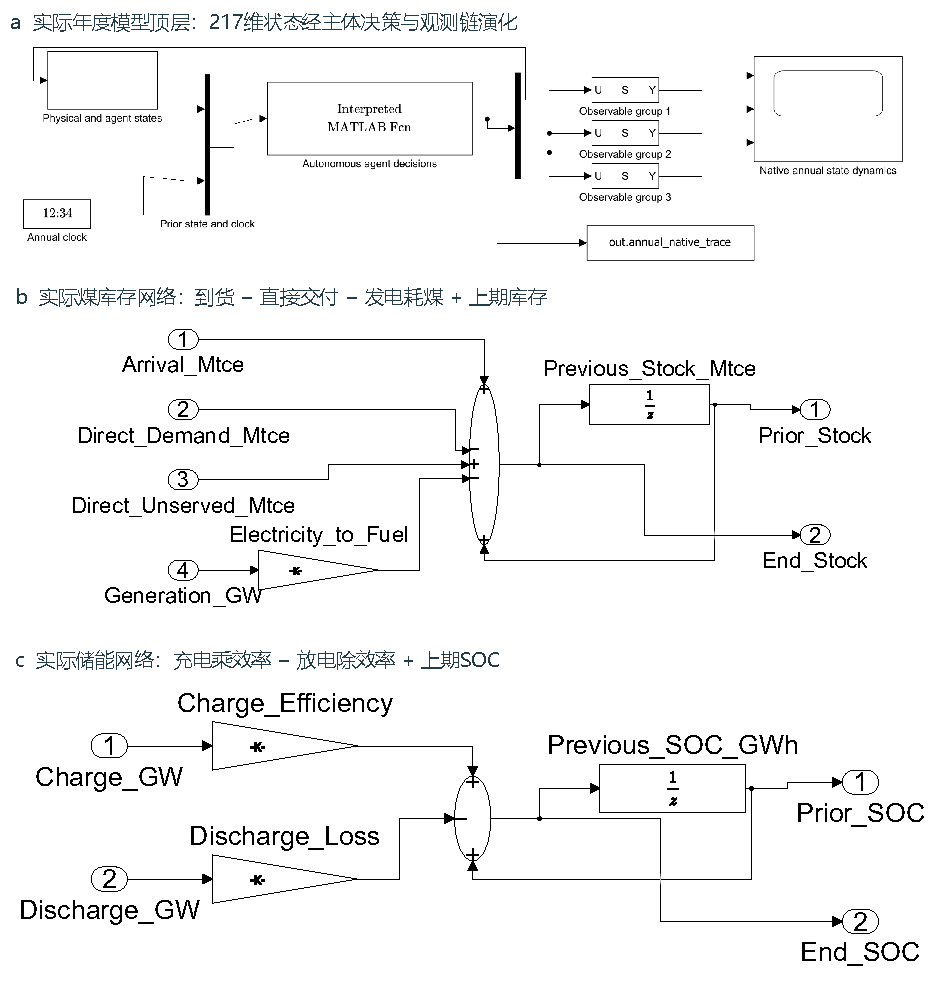
\includegraphics[width=\linewidth]{figures/native_v9_resource_conservation.pdf}\caption{实际Simulink工程的全景与守恒局部。a为年度217维状态模型的真实顶层封装，主体与12类资产15槽队列在决策函数内实现；b—c为煤库存与储能的原生矢量导出，分别按G/(8141$\eta$) Mtce/小时和$\eta_c$·充电$-$放电/$\eta_d$更新。中文说明位于原图外，Unit Delay保存上一小时状态。}\end{figure}

新物理网络在继承供应和付费补库下分别连续执行2160小时，与已执行输出逐列核对49个通道，并从导出CSV独立重建电力、燃料、SOC与债务账；最大电力平衡残差为$1.23\times10^{-11}$ GW。年度实现另对15组状态演化核对。新增保供修复（方案Ⅰ）在相同Simulink年度模型中实际完成2025—2060年演化，仅输入观察初态、固定参数与常量政策，由原生模型逐年产生217维状态和12类投资动作。36年共7,812个状态值、4,752个原始指标及432次投资动作与独立Python实现核对，最大归一化差为$3.64\times10^{-12}$；建设队列移位、投产与退役逐项相符，三燃料、电力及资本账独立闭合。该实现检验与前述历史误差分别报告：前者检查状态方程和实现，后者检查历史资料下的组件表现。

\begin{table}[H]\centering\caption{历史诊断、物理验证与原生实现的分层检验}
\begin{tabularx}{\linewidth}{p{.19\linewidth}XX}\toprule
检验层次 & 方法与对象 & 已完成证据\\\midrule
历史与行为 & 各训练起点以前资料校准共享预期及资产组件，条件给定已实现GDP & 一年/三年电力MAPE为1.713\%/3.992\%；近期净增基线为2.306\%/2.452\%\\
数学与物理 & 逐时平衡、库存、SOC、爬坡及负荷债务；线性规划原域与对偶条件 & 电力平衡最大残差$1.23\times10^{-11}$ GW；联合约束与末态证书按实际成功记录核查\\
软件实现 & MATLAB/Simulink与Python年度状态；AnyMath与Python各自闭环 & 年度最大归一化差$3.64\times10^{-12}$；1800个小时缺供差最大$2.3\times10^{-13}$ GW\\
\bottomrule\end{tabularx}\end{table}
各组对照采用相同初态和声明的信息条件，先用既有路径核对实现，再完整执行固定比较组；输入、原始结果与全部失败状态列于附录及支撑材料。年度控制在48组开发设计中选择，另48组拉丁超立方设计以种子20261019独立生成，控制固定后只检验一次，未据此再调参。工程设计范围与历史误差、软件一致性分别解释。

\subsection{AnyMath参数干预、小时重优化与连续恢复}
AnyMath实现采用“读取原生状态—求解24小时协调问题—执行首小时动作—原生网络推进状态”的循环。Julia/HiGHS在每小时重新优化发电、两类储能、移峰及未满足服务等18项动作，原生Sum、Gain和Unit Delay网络计算三燃料库存、两储能SOC、移峰债务及两机组记忆；下一次优化读取这些原生末状态\cite{anymath_docs}。修改冲击强度、持续时间、补库方式或储能功率后，从同一初态建立新会话，旧轨迹保留其参数身份。

为直观展示两次冲击与中间恢复，另设360小时工程设计：冲击区间为$[48,96)$与$[192,240)$，合同在冲击退出12小时后开始补库；系统采用折中2060快照。短设计与前述2160小时试验分别覆盖不同事件持续期，缺供和恢复结果各按所属设计报告。五组参数均在平台内完成360次逐时优化与原生状态推进，共享24小时完美前瞻，求解状态逐小时导出。

\begin{figure}[H]\centering
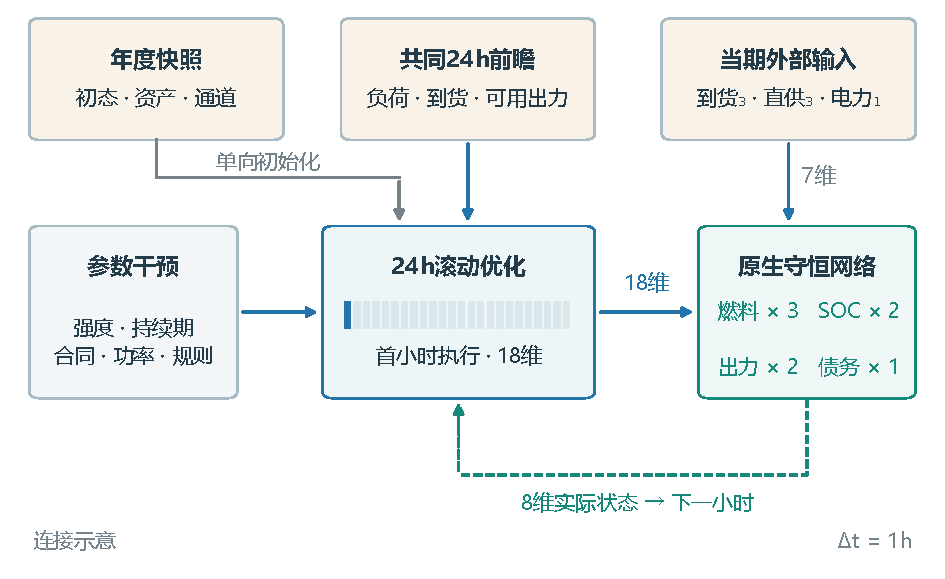
\includegraphics[width=\linewidth]{figures/native_closed_loop.pdf}
\caption{已实现小时系统的分层连接。年度快照单向提供初态、资产和通道能力，优化器与原生网络使用同源初态；共同24小时前瞻进入滚动优化，只执行首小时18维动作。7维当期外部输入与动作进入原生守恒网络，三燃料库存、两类SOC、两类热机出力记忆及一项移峰债务共8维实际状态反馈至下一小时，步长1h。此图为连接示意；箭头宽度不表示流量。}
\label{fig:native_closed_loop}\end{figure}

\begin{figure}[H]\centering
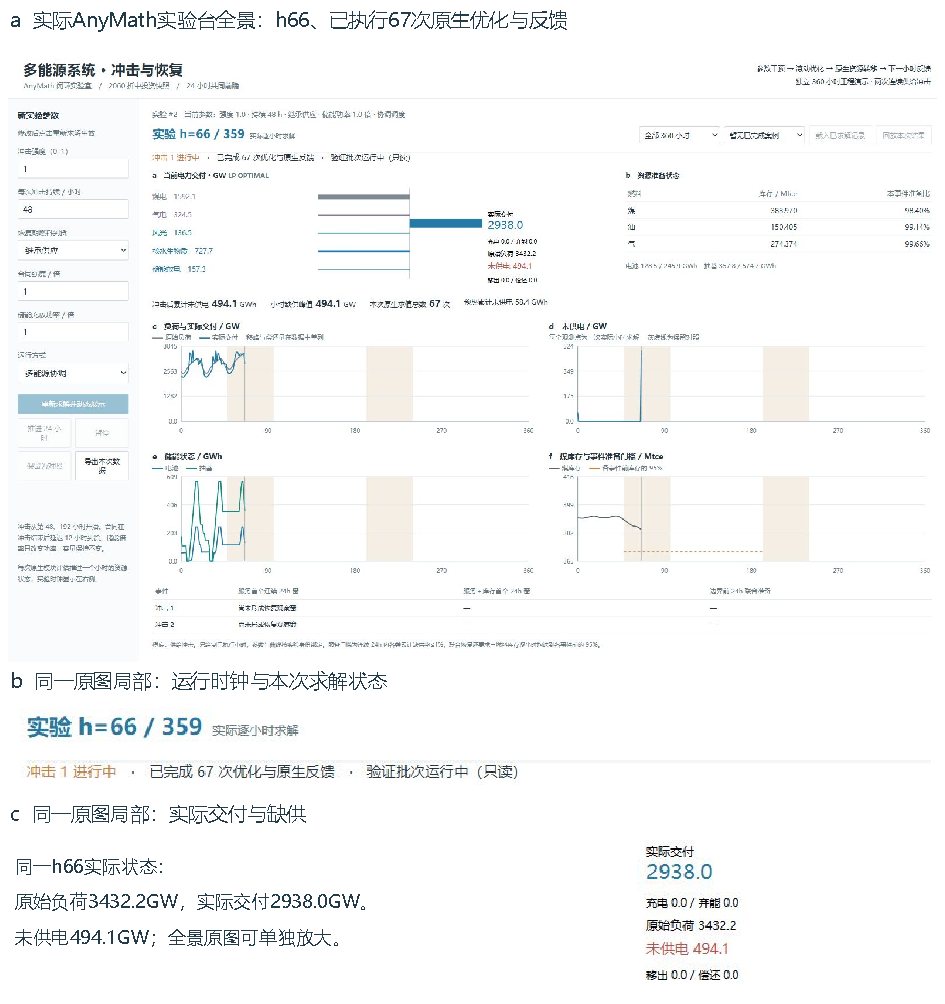
\includegraphics[width=\linewidth]{figures/native_anymath_v10_live.pdf}
\caption{同一h66的AnyMath真实全景与局部放大。参数控制、能流、库存/SOC、六视图和恢复表来自同一原图；b显示h66/359及已执行67次优化与原生反馈，c显示实际交付2938.0GW和缺供494.1GW。全景未拼接不同时刻，原始高清图随支撑材料提供。}
\label{fig:anymath_v10_live}\end{figure}

\begin{table}[H]\centering\caption{AnyMath闭环设计实验的实际结果（均为360小时全段）}
\begin{tabular}{lrrr}\toprule
方案 & 未供电/TWh & CO$_2$/Mt & 资源费/亿元\\\midrule
协调基准 & 5.228 & 439.7 & 4,548.2 \\
减轻冲击 & 0.058 & 393.7 & 4,350.6 \\
提高储能功率 & 5.170 & 436.3 & 4,548.5 \\
合同补库 & 5.228 & 439.7 & 5,103.7 \\
分散策略 & 8.192 & 440.9 & 4,548.6 \\
\bottomrule\end{tabular}\end{table}
\noindent 资源费按到货、库存领用、非化石运行、储能、移峰、库存持有与合同溢价记账，不含缺供惩罚、碳价转移及增功率工程投资。未供电含初始化阶段，前述2160小时剔除预热的指标另行报告。

\textbf{提高功率改变缺口时序，补库改变跨事件资源准备。}在能量容量不变时，将储能功率提高50\%，第66小时两类储能多交付78.634 GW，主窗缺供峰值由494.1降至415.5 GW。峰后缺口回补与削峰改善各为0.681 TWh，主窗累计未供电仍为5.170 TWh；全段减少的0.058 TWh来自前48小时初始化。因此，峰值改善与累计能量改善应分别核算。

应急合同在冲击退出12小时后开始追加到货，期末煤库存增加10.623 Mtce，而全段缺供仍为5.228 TWh。这一对照表明，新增资源在本组事件中主要转为库存准备，不能仅由采购量推断电力增发；其作用应继续沿恢复窗口和事件边界检验。

联合恢复须在连续24小时内满足各服务合计缺供率不超过1\%、三库存逐小时不低于事件前95\%。以下按本次条件轨迹比较首次确认、再跌破和观察边界，未确认者保留右截尾。

第1次冲击后，协调基准在第119小时确认首个合格窗口，又在第146小时重新跌破库存门槛。到观察边界，基准与合同方案的煤库存分别为各自冲击前的94.74\%和95.93\%；最后24小时联合准备分别为未达标与达标。

第2次冲击后，协调基准在第263小时确认首个合格窗口，又在第269小时重新跌破库存门槛。到观察边界，基准与合同方案的煤库存分别为各自冲击前的94.05\%和95.72\%；最后24小时联合准备分别为未达标与达标。

在本次条件轨迹中，合同补库使两次观察边界的联合准备均转为达标，累计未供电保持不变；资源准备与当期电力交付分别响应不同约束。


\begin{figure}[H]\centering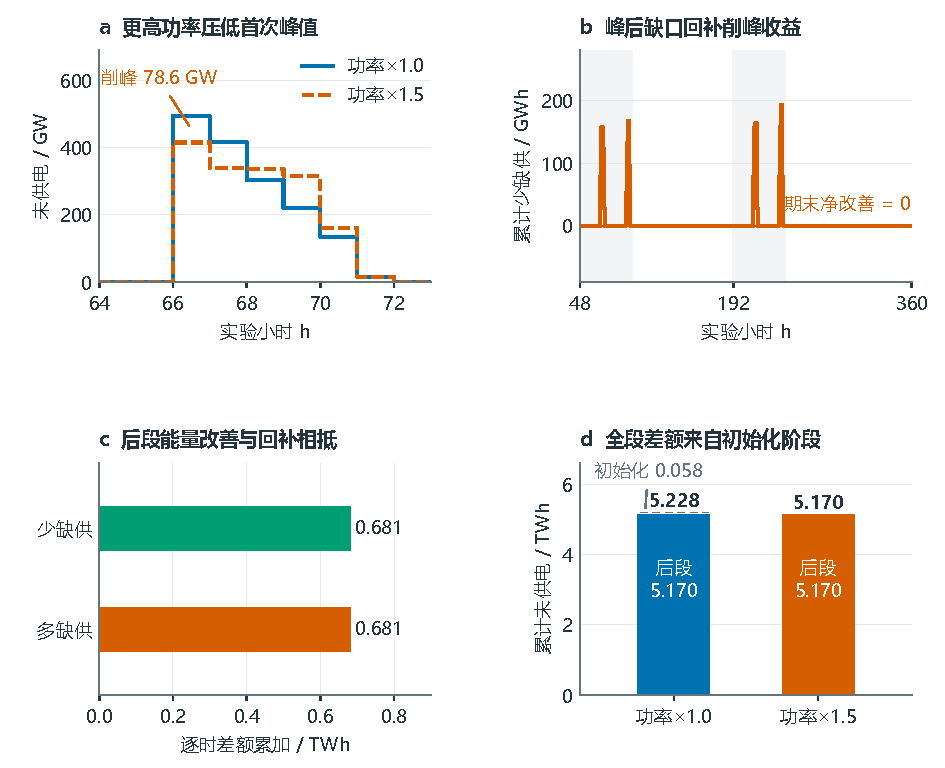
\includegraphics[width=\linewidth]{figures/figI_power_energy_accounting.pdf}
\caption{储能功率与能量缺口的分离。放电功率增加改变逐时缺口分布，后段缺供增减能量相互抵消；初始化阶段另列，全部功率与能量保持相应单位。}\label{fig:figI_power_energy_accounting}\end{figure}

\subsection{恢复定义与完整路径检验}
固定已执行轨迹，将连续窗口设为12、24、48小时，库存门槛设为90\%、95\%、99\%，各服务缺失门槛设为0.5\%、1\%、2\%，共重算270个事件定义。默认定义逐项复现原10个事件，计算前后调度动作保持原值。定义$\kappa_{e,W}=\min_{h\in[T_e-W,T_e),f}S_{f,h}/S_{f,\mathrm{pre}}$，其中$T_e$为事件观察边界，$S_{f,\mathrm{pre}}$为该次冲击前库存；$\kappa$即边界前$W$小时所有燃料的最小库存比。在服务合格时，库存要求不超过$\kappa$即可维持该窗口准备。

两次事件的24小时库存底线，基准分别为94.74、94.05\%，合同分别为95.82、95.65\%。95\%要求处于两方案的分界区间，区分了当期服务与持续准备；90\%和99\%规则分别对应更宽松和更严格的资源要求。

另以独立SciPy/HiGHS新执行五条各360小时完整闭环路径，两实现各自反馈本实现的实际状态。1800个逐小时缺供差的最大值为$2.3\times10^{-13}$ GW，累计缺供及10个事件的默认恢复判定、再跌破时刻一致。两实现的SOC、机组输出与偿还时点存在分支；这组完整路径比较与同状态最优目标核验共同支持本组服务和准备结论，实际轨迹仍保留其求解器身份。

\subsection{用更强的局部规则识别协调的增量价值}
原分散规则以需求减非化石可用出力形成储能净负荷，正值放电、负值充电。冲击期间，非化石出力不足使其难以利用煤气电余量充电。为检验协调在更强规则下的作用，增加“可达全电源余量局部”规则：以当期真实热机记忆出发，逐时按爬坡和可用上限递推煤气电可达出力，连同非化石可用出力计算储能净负荷；沿用原贪心储能顺序、效率和SOC约束，再由同一市场调度器执行。该规则使用同样24小时前瞻、资产、外部输入和资源账。
\begin{table}[H]\centering\caption{更强局部规则与协调的完整路径比较}
\begin{tabular}{lrrrr}\toprule
规则 & \shortstack{主窗缺供\\GWh} & \shortstack{主窗峰\\GW} & \shortstack{全段资源费\\十亿元} & \shortstack{全段CO$_2$\\Mt}\\\midrule
协调/原功率 & 5169.910 & 494.114 & 454.819 & 439.721 \\
可达余量局部/原功率 & 5279.366 & 494.114 & 459.893 & 447.447 \\
协调/1.5倍功率 & 5169.910 & 415.480 & 454.845 & 436.283 \\
可达余量局部/1.5倍功率 & 5222.077 & 415.480 & 460.277 & 444.789 \\
指定非化石局部/原功率 & 8133.428 & 651.383 & 454.855 & 440.877 \\
\bottomrule\end{tabular}
\end{table}
原功率下，协调相对可达余量局部规则减少缺供109.455 GWh（2.073\%）；1.5倍功率下减少52.167 GWh（0.999\%），两组各自的峰值相同。36.4\%的原结果对应指定非化石局部规则，更强基线下的增量来自联合安排储能、发电与负荷偿还。原功率/1.5倍功率下，协调资源费分别少50.737/54.324亿元、燃烧CO$_2$少7.726/8.506 Mt。终态也随策略改变：协调末SOC接近零，可达余量局部规则末电池与抽蓄均充满，合计820.638 GWh；费用已按相同0.32百万元/GWh计入SOC净领用，燃料库存另按同一价格计价。费用和排放随实际轨迹比较，终态准备程度由独立库存与SOC账同时呈现。

\subsection{相同期末储能电量下，协调收益仍保留}\label{sec:common-terminal}
原比较的协调路径期末储能接近零，强本地规则期末充满。保持四种控制与全部外部输入，新增共同终点要求：第360小时边界，电池与抽蓄均达到各自满容量，合计820.638 GWh。仅在滚动窗口触及真实终点时改变两个末SOC边界；

共同终点的干预仅在最后24小时进入规划，四臂第0—335小时全部状态与动作逐值相同。两条强本地路径全程不变；两条协调路径在后段减少放电并增加充电，额外煤气发电分别为774.727、791.650 GWh，完整路径缺供均不增加。电池和抽蓄电量统一后，实际燃料库存与热机出力继续逐项报告。
\begin{table}[H]\centering\caption{共同满电终点下，强本地规则减协调的配对差}
\begin{tabular}{lrrrr}\toprule
功率条件 & \shortstack{主窗缺供\\GWh} & \shortstack{主窗峰值\\GW} & \shortstack{全段物理费\\亿元} & \shortstack{全段CO$_2$\\Mt}\\\midrule
原功率 & 109.455 & 数值零 & 50.750 & 7.088 \\
1.5倍功率 & 52.167 & 数值零 & 54.007 & 7.891 \\
\bottomrule\end{tabular}
\smallskip\par\noindent 主窗为h48—359，全段为h0—359；峰值原始差约$5.7\times10^{-13}$ GW，展示阈值$10^{-8}$ GW。
\end{table}
原功率与1.5倍功率下，协调的缺供、物理资源费用与CO$_2$改善均保留，峰值各自相同。物理费沿用燃料到货与净库存、非燃料运行、储能循环、移峰、SOC净领用及库存持有账。共同终点使原SOC净领用估值项减少262.604百万元；两协调路径的其他运行资源费增加261.344、294.261百万元，净物理费分别变化$-1.260$、$+31.656$百万元。增购末电量形成资产，运行补电支出与净资源费据此衔接。
\begin{figure}[H]\centering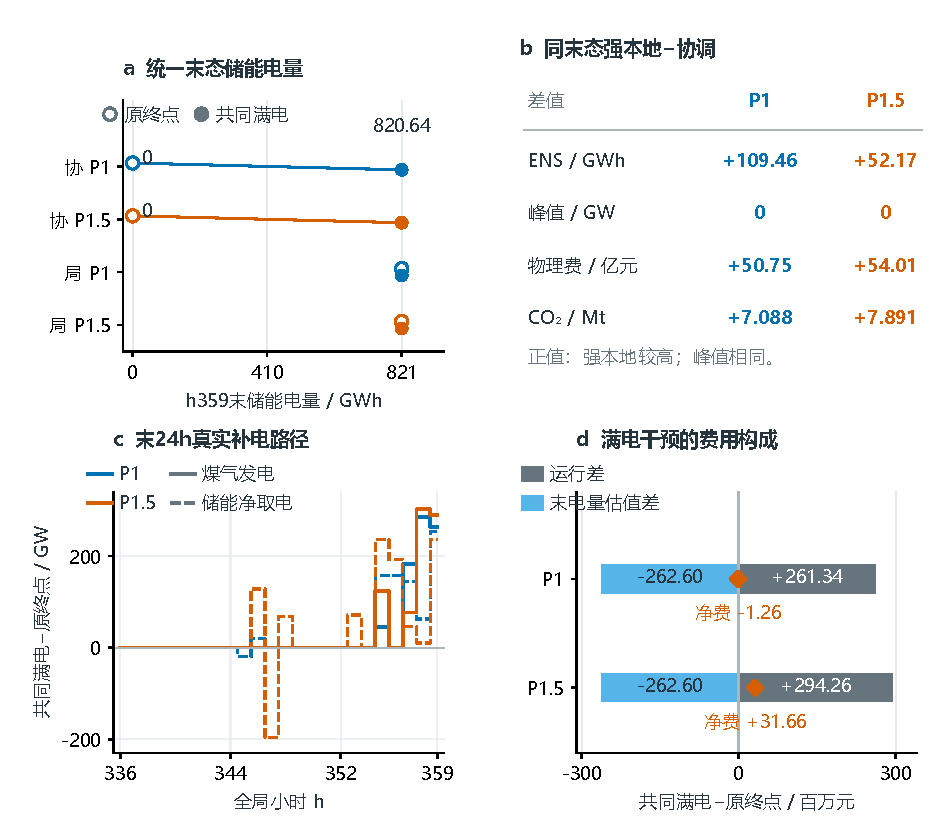
\includegraphics[width=\linewidth]{figures/figO_common_terminal_storage.pdf}\caption{共同满电终点下的实际补电、收益与计价。ENS和峰值取h48—359，费用及排放取完整360小时；共同满电约束进入h336—359。两功率仅P不同，能量容量、初始50\%电量和24小时前瞻相同；费用含0.32百万元/GWh末电量净领用估值，不含缺供罚金和碳价，末燃料与热机出力仍可不同。}\end{figure}

\subsection{事件信息改变动作与费用，服务结果另行检验}
保持24小时优化窗口和正常工程日型已知，只改变事件状态的可见时长$L=1,6,24$小时；超过可见部分，以最后一个已知事件状态延续。真实执行始终使用实际当小时事件，三条原策略各执行三种信息条件，共9条360小时路径。每条路径继承自身实际库存、SOC、爬坡记忆与债务，常态日型与事件预见性分别设置。

三种信息条件下，各原策略主窗累计缺供和峰值数值一致；动作并未全部相同。$L=1$相对24小时，协调、增功率协调和指定非化石局部规则分别有41、44、14个小时动作改变，全段资源费用分别增加1.544、2.464、1.619亿元。协调首次库存再跌破由第146小时前移至第145小时，服务窗口仍在第119、263小时确认。该组瓶颈限制了服务指标对信息变化的响应，信息价值同时体现在实际动作、资源领用与准备时点上。

\subsection{完整事件设计给出动作的优势区间}
固定上述五条控制器，以相位$\phi\in\{0,3,6,9,12,15,18,21\}$小时、事件持续期$d\in\{12,24,48,72\}$小时组成32个格点。两次冲击从$48+\phi$、$192+\phi$开始，其他事件强度、进口和需求扰动、360小时时轴及24小时前瞻保持原值。每格完整执行五条路径，160组共57,600小时；相位同时改变冲击与负荷/风光日型、绝对偿还时点的相遇关系，持续期改变事件剂量，因而各格用于工程设计条件的比较。

\begin{figure}[H]\centering
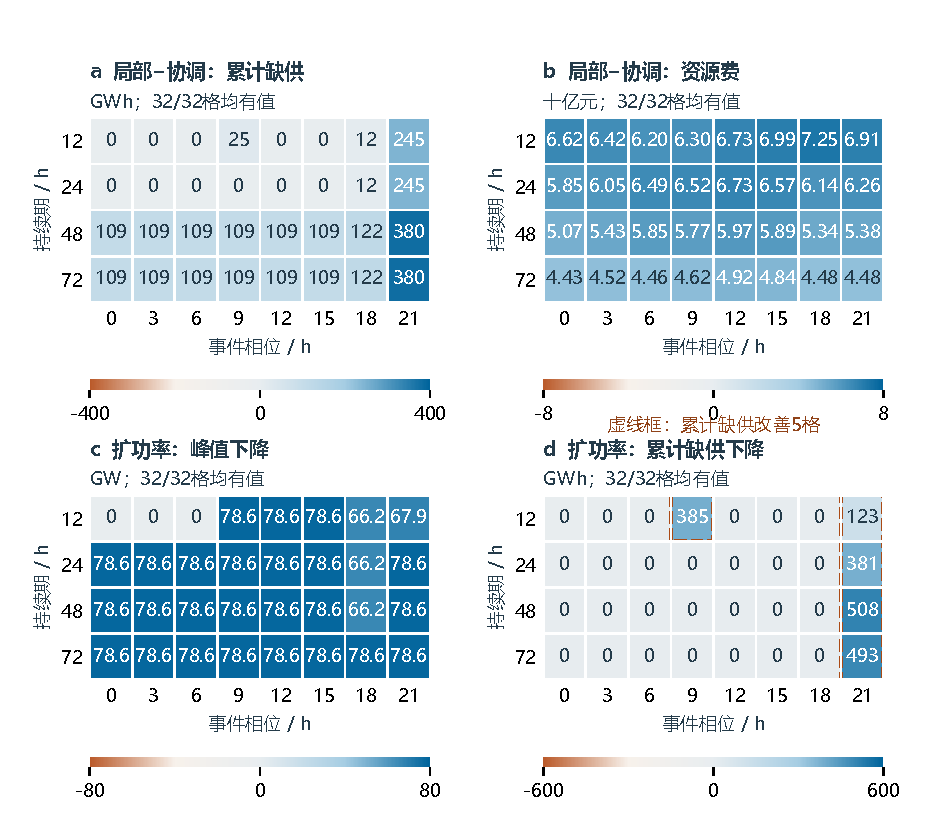
\includegraphics[width=160mm]{figures/figM_event_advantage_domain.pdf}
\caption{32格事件条件下的完整优势域。a—b为原功率下可达全电源余量局部减协调；c—d为协调原功率减1.5倍功率，能量容量不变。虚线框仅标5个累计缺供改善格，27格为有效数值零，不能统一解释为已达夜间守恒下界。主窗h48—359；各面板单位内绝对差$\le$$10^{-8}$显示0，原值128格完整保留，费用含净库存与SOC领用估值。}
\label{fig:event-advantage}\end{figure}

对可达余量局部规则，原功率协调在21/32格减少主窗缺供、11格数值相同，改善范围0—379.620 GWh；1.5倍功率下分别为19格改善、13格相同，改善0—422.201 GWh。原功率32格资源费均下降44.296—72.539亿元、燃烧CO$_2$少5.041—11.331 Mt，终态SOC差保持上述方向。全部格点展示了收益的大小与条件。

增加50\%储能功率在29/32格削减小时缺供峰值，最大78.634 GW；累计缺供仅在5/32格减少，范围0—508.270 GWh，另外27格数值相同。5个改善格为相位9小时/持续12小时，以及相位21小时/持续12、24、48、72小时。相位9、持续12小时格在第66—68小时多交付192.538 GWh；冲击第69小时结束后，可用能力盈余足以偿还负荷，额外交付得以保留为累计改善。原相位0、持续48小时格则将同一可用储能能量重新分配，主窗缺供总量相同。功率扩充能否进一步减少能量短缺，取决于功率受限时仍有可用能量，以及事件退出后能否无新增缺供地偿还先前负荷。各格的改善比例用于这32种设计条件，事件发生概率需由独立资料建立。

\subsection{储能时长依据与单参数挑战}
国家能源局报告给出2024年底新型储能73.76 GW、168 GWh、平均2.3小时，统计涵盖多种新型储能技术\cite{nea_storage_2025}。本文基年采用73.76 GW功率，并以4小时电池、6小时抽蓄作为工程配置；4小时也属于NREL储能技术经济比较的代表配置\cite{nrel_atb_storage}。为检验能量配置对运行结论的影响，固定折中2060资产和全部控制，将电池容量从原功率乘4小时改为原功率乘2.3小时，初始SOC仍为各自容量的50\%。同一时长内增加功率保持能量容量不变，抽蓄保持6小时；五规则各执行两时长，共10条完整路径、3600小时。
\begin{table}[H]\centering\caption{电池时长变化下的主窗缺供}
\begin{tabular}{rrrrr}\toprule
\shortstack{电池时长\\h} & \shortstack{协调原功率\\GWh} & \shortstack{可达局部原功率\\GWh} & \shortstack{协调1.5倍\\GWh} & \shortstack{可达局部1.5倍\\GWh}\\\midrule
4.0 & 5169.910 & 5279.366 & 5169.910 & 5222.077 \\
2.3 & 5566.564 & 5676.019 & 5566.564 & 5618.731 \\
\bottomrule\end{tabular}
\end{table}

电池由4小时减为2.3小时，协调在两种功率下主窗缺供均增加396.654 GWh，约为主窗原始需求的0.0434个百分点；两种功率协调的峰值仍为494.114/415.480 GW，累计缺供仍相同。2.3小时下，协调相对可达余量局部规则依然分别少缺供109.455/52.167 GWh；在1.5倍功率下还将峰值由465.778降至415.480 GW，较少可用能量使规则间的削峰差异显现。能量配置影响累计交付，功率配置影响逐时交付，两者在本组设计中分别显现。该试验只改变小时电池能量与其初始SOC，年度投资路径和资本费用继续按原组合报告。

\subsection{累计缺供的离线最优参照与剩余调度空间}
固定相位0/21小时、原功率/1.5倍功率、末SOC自由/共同满电八组条件，每组先复现24小时滚动路径，再固定其实际前48小时，从第48小时完整状态一次优化剩余312小时。原燃料、爬坡、容量、效率及13个绝对日末偿债条件全部保留，三种直接燃料服务全额交付。该离线参照同时获得真实后续输入并改变优化方式，用于识别固定资产下的可达边界。

先最小化累计缺供$U$，再在$U\le U^*+10^{-6}$ GWh下最小化物理资源费。8条滚动与8条离线共执行5760小时实际状态转移、2896次LP；原矩阵、解与对偶全部保存。八组滚动缺供与第一阶段最小值均数值相同，滚动值与对偶下界的最大绝对间隙小于$1.2\times10^{-11}$ GWh。第二阶段增加的约1 kWh来自预定容差。

\subsection{用四段夜间守恒解释能量瓶颈}
对结束于绝对日末的窗口$W=[a,b)$，债务$Z_b=0$、$Z_a\ge0$给出$\sum_W(repay-out)=Z_a\ge0$。储能满足$S_b-S_a=\eta_c\sum ch-\sum dis/\eta_d$，结合$0\le S\le E$与$\eta_c\eta_d\le1$，得到$\sum_W(dis-ch)\le\eta_dE$。再用发电可用上限$A$及电力平衡，得到
\begin{equation}
\sum_{t\in W}ENS_t\ge\left[\sum_{t\in W}\left(D_t-\sum_gA_{g,t}\right)-\sum_s\eta_{d,s}E_s\right]_+.
\label{eq:night-cut}
\end{equation}
每窗允许从满电开始，已放宽了真实燃料、爬坡与前期充电限制；四个互不重叠窗口的下界可以相加。图\ref{fig:energy-cut}把可用发电后的总缺口拆成最多可交付储能与不可消除的缺供。

\begin{figure}[H]\centering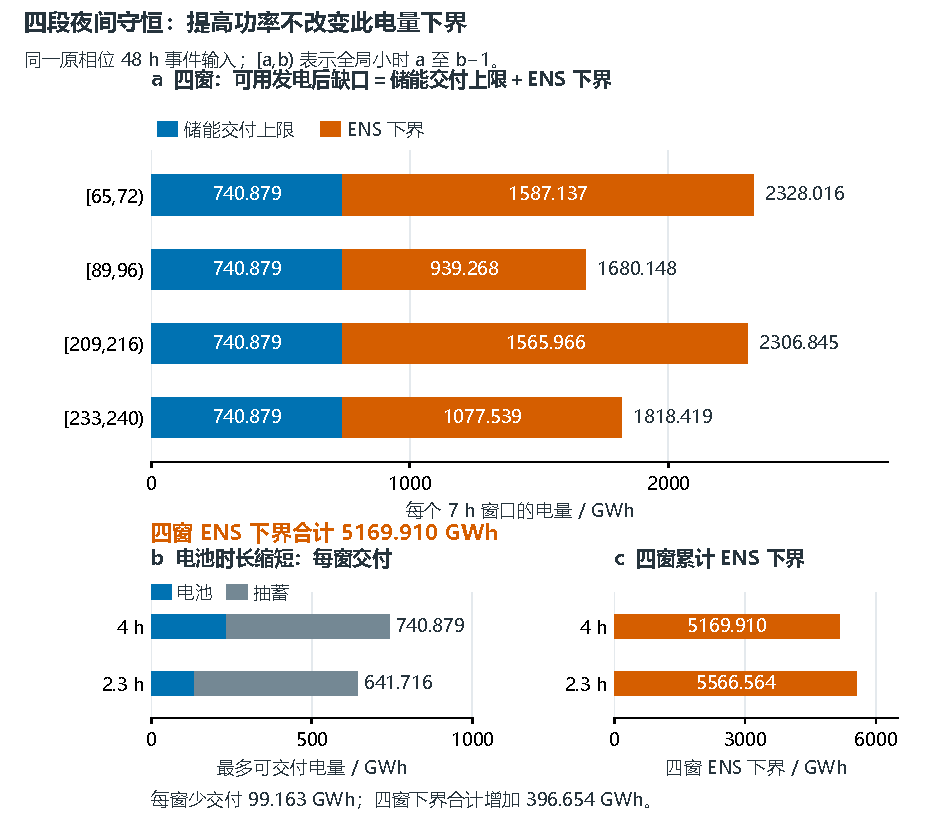
\includegraphics[width=160mm]{figures/figR_energy_conservation_floor.pdf}
\caption{原相位四段夜间的能量守恒下界。四个不重叠7小时窗均结束于日末偿债点，每窗允许满电开始，最大储能交付$\sum_j\eta_{d,j}E_j$；移峰不能净移出窗口。下界合计5169.910GWh，功率增加50\%而E不变时下界不变；电池由4小时减至2.3小时使四窗交付减少396.654GWh。结论限该原相位、既定容量与日末偿还规则，完整14路径56窗另表。}\label{fig:energy-cut}\end{figure}

这一结果解释了原48小时设计：调度已到达累计电量边界，增加功率仍可改变缺口的小时分布，增加可交付能量才可能下移该边界。32格事件试验中的5个能量改善格则具有不同的功率受限与事后偿还条件，按各自实际路径判断。

\subsection{多目标约束的费用边界与等费保峰排程}
在同一缺供边界上，分别增加燃烧排放不超过原滚动值、每小时缺供不超过原滚动峰值，以及两者共同约束；八组各三臂共24次LP和8640小时物理转移。沿用同一实际前缀、原矩阵、资源价格和缺供容差。记原二阶段可行域为$F_0$，碳、峰、联合约束域为$F_C,F_P,F_{CP}$，相应最小费用为$v_0,v_C,v_P,v_{CP}$。原滚动向量在四域均可行，故
\begin{equation}
v_0\le v_C\le v_{CP}\le v_R,\qquad v_0\le v_P\le v_{CP}\le v_R.
\end{equation}
完整24臂给出更细的结果：八组均有$v_P=v_0$及$v_{CP}=v_C$的数值等价关系，最大费用差小于$5.9\times10^{-11}$百万元。因此，先前保存的六条最低费用解虽提高了缺供峰值，另有等费最优解可把峰值控制回原水平。峰值升高来自当次最优排程的选择，并非这些条件下省费所必需。

无附加碳帽时，保住峰值仍可节省12.861—20.924亿元，但排放增加10.721—12.427 Mt。再守住排放后，六组只剩698.316—2738.648万元节约，另两组为数值等费；两组原始差约3.166元，低于10元费用证书容差。排放约束才明显压缩本组降费空间。

\begin{figure}[H]\centering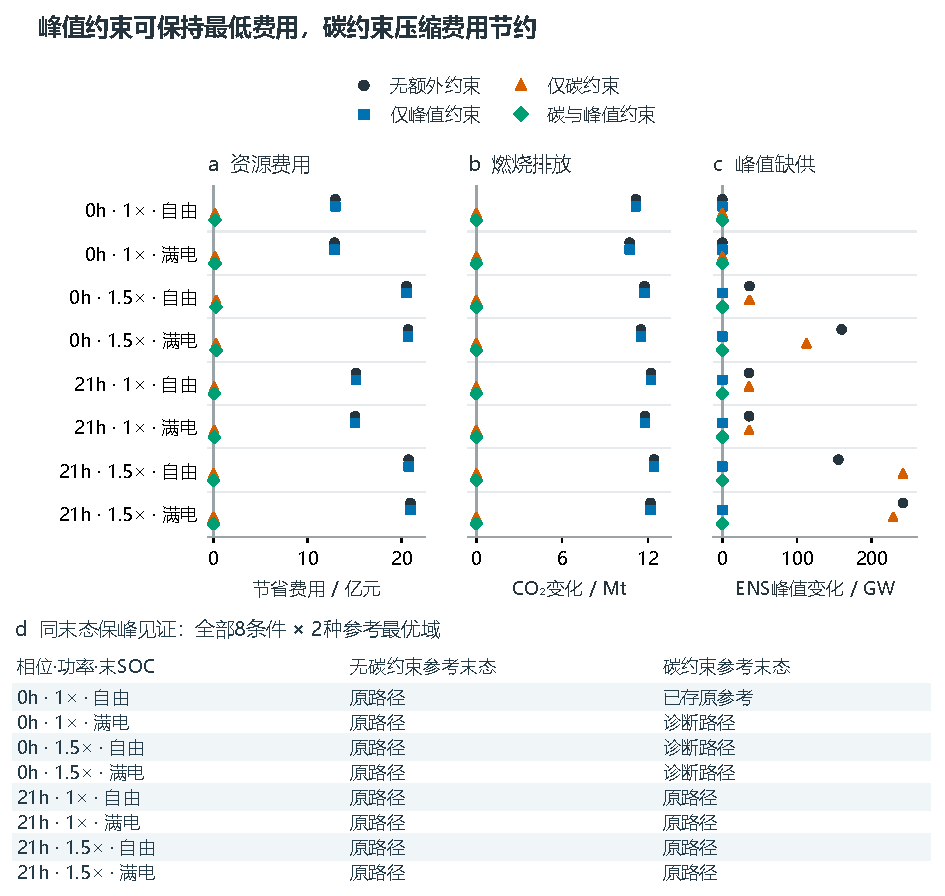
\includegraphics[width=160mm]{figures/figS_joint_dispatch_constraints.pdf}
\caption{同一缺供边界上的四类最优排程。a—c按全部八条件相对对应滚动路径比较费用、排放、峰值，主窗h48—359；实际前48小时固定，后312小时一次优化。ENS容差$10^{-6}$GWh，物理费含净SOC领用与持有费，不含碳价和缺供罚金。d保留全部16个同末态保峰见证，固定各自最优解的三燃料、两SOC与两热机末出力；“已存原参考”表示直接验证既有排程，$\le$10元不作收益。}\label{fig:joint-dispatch}\end{figure}

保峰是否占用了期末资源，还需在相同末态下比较。固定各自参考最优解的三种燃料库存、两项SOC及煤气末出力，16个条件均有费用数值等价的保峰排程；其中15个条件由新增成功解覆盖，另一个由原参考排程及其原域证书直接确认。完整尝试及求解器状态见附录，同末态比较的对象始终是各自参考解。

这一比较将操作目标落实为可检查的约束：累计能量边界由供给与可交付储能决定；同一边界内的小时缺口可重新分配；费用优化还必须同时查看排放与期末准备。资源费仍逐项核对燃料领用、非燃料运行、循环、移峰、净SOC领用和库存持有；各电源发电与费用分解、原最低费用图及全部末态列于附录。

\begin{table}[H]\centering\caption{关键工程参数的依据与作用}
\begin{tabularx}{\linewidth}{p{.18\linewidth}p{.25\linewidth}X}\toprule
参数 & 采用值 & 依据及在模型中的作用\\\midrule
储能配置 & 电池4小时，抽蓄6小时 & 工程配置；以官方2024多技术储能平均2.3小时增算单参数挑战\\
热机上爬坡 & 煤0.15、气0.70倍额定功率/小时 & 聚合工程约束，逐时限制由真实上期出力可达的本期出力\\
初始燃料储备 & 2024年按45天年消费初始化 & 年度初态设计；后续年度积累，小时层读取所选年份实际年末库存\\
联合恢复 & 服务缺失至多1\%，库存至少事件前95\%，持续24小时 & 本文操作判据；固定初始与同小时无事件库存另列参照\\
\bottomrule\end{tabularx}\end{table}
\FloatBarrier
